\documentclass[aspectratio=169,11pt]{beamer}
\usepackage[utf8]{inputenc}\usepackage[T1]{fontenc}
\usepackage[spanish,es-nodecimaldot,es-noshorthands]{babel}
\usepackage{amsmath,amssymb,booktabs,graphicx,listings}
\definecolor{navy}{HTML}{183754}
\definecolor{accent}{HTML}{B65F29}
\usetheme{default}
\setbeamertemplate{navigation symbols}{}
\setbeamertemplate{footline}{\hfill\insertframenumber/\inserttotalframenumber\hspace{1em}\vskip4pt}
\setbeamercolor{frametitle}{fg=navy}
\setbeamercolor{structure}{fg=navy}
\setbeamercolor{alerted text}{fg=accent}
\setbeamerfont{frametitle}{size=\Large,series=\bfseries}
\setbeamersize{text margin left=8mm,text margin right=8mm}
\newcommand{\source}[1]{\par\vfill{\tiny\color{gray}#1\par}}
\lstset{basicstyle=\ttfamily\scriptsize,breaklines=true,columns=fullflexible,
 literate={∧}{{$\land$}}1 {≤}{{$\le$}}1 {≥}{{$\ge$}}1 {ℝ}{{$\mathbb R$}}1 {→}{{$\to$}}1 {≠}{{$\ne$}}1}
\newcommand{\threshold}{0.640}
\newcommand{\betaZero}{0.130}
\newcommand{\betaOne}{-0.085}
\newcommand{\riskMin}{8.89}
\newcommand{\riskMax}{23.80}
\newcommand{\effortMin}{0.224}
\newcommand{\effortMax}{0.400}
\newcommand{\cohortSlope}{0.130}
\newcommand{\stockSlope}{-0.034}

\begin{document}

% Exposición estimada: 30 segundos.
\begin{frame}[plain]

\begin{center}
{\LARGE\color{navy} Precio relativo del crédito\\[.3em]y morosidad futura}\par\bigskip
{\large Evaluación óptima y composición de la cartera}\par\bigskip
Fabián Matías Galarza Chumbe\\
Línea B. Curso: IA y modelación económica\\
11 de noviembre de 2026\par\par\medskip
\href{https://github.com/fgalarzac/ai-project}{github.com/fgalarzac/ai-project}
\end{center}
\end{frame}

% Exposición estimada: 60 segundos.
\begin{frame}{El problema del supervisor}

Un banco publica el precio de sus operaciones nuevas antes de observar su desempeño.
\par\medskip
\begin{itemize}
\item Una señal útil permitiría priorizar la revisión de carteras.
\item La tasa también contiene fondeo, costos y margen.
\item El atraso de toda la cartera mezcla préstamos de distintas edades.
\end{itemize}
\par\medskip
\textbf{Objeto de interés:} el contenido informativo de una brecha de precios frente a bancos comparables.
\source{\href{https://www.sbs.gob.pe/app/stats/Metodologia/Metodologia_TI_promedio.pdf}{SBS, metodología, sección 3}. \href{https://doi.org/10.1023/B:FINA.0000003322.43105.33}{Morgan y Ashcraft (2003)}.}
\end{frame}

% Exposición estimada: 70 segundos.
\begin{frame}{Heterogeneidad que exige comparar bien}

CAR significa cartera de alto riesgo: vencidos, cobranza judicial,
refinanciados y reestructurados. El ajuste incorpora castigos recientes.
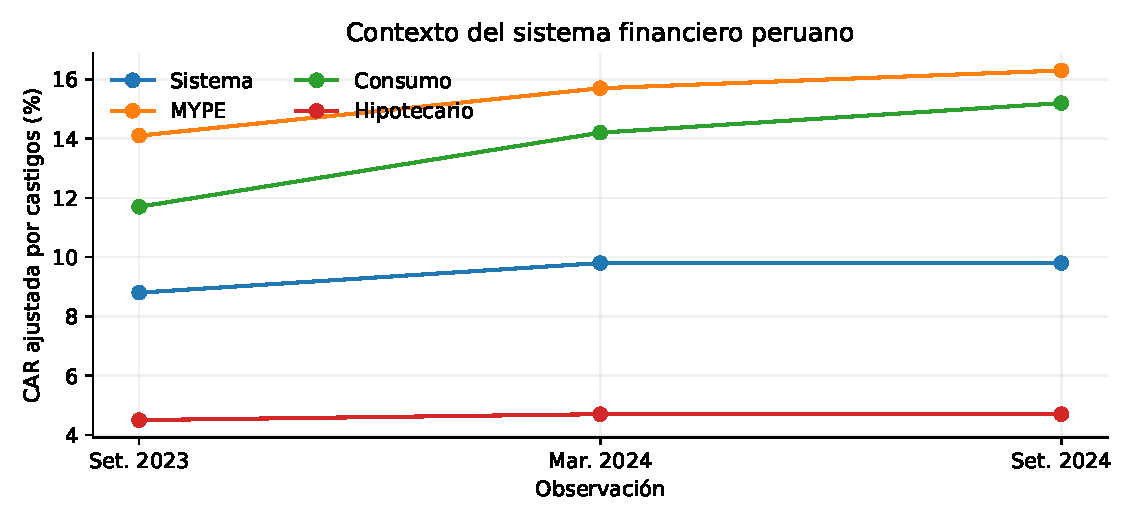
\includegraphics[width=.87\linewidth,height=.55\textheight,keepaspectratio]{../code/figures/public_context.pdf}
\par\small MIPE: micro y pequeña empresa. CAR ajustada: distinta de mora contable y de atraso mayor de 90 días.
\source{\href{https://www.bcrp.gob.pe/docs/Publicaciones/Reporte-Estabilidad-Financiera/2024/noviembre/ref-noviembre-2024.pdf}{BCRP, Reporte de Estabilidad Financiera, noviembre de 2024, cuadro 2.2, p. 21}. Sistema financiero, no solo banca múltiple.}
\end{frame}

% Exposición estimada: 50 segundos.
\begin{frame}{Pregunta y resultado condicionado}

\textbf{Pregunta:} ¿cuándo una tasa por encima de los pares anticipa mayor morosidad?
\par\medskip
\begin{itemize}
\item En el interior, el riesgo nuevo aumenta si selección supera a evaluación.
\item Las restricciones cambian esa regla.
\item En el saldo total, la composición puede invertir el signo.
\end{itemize}
\par\medskip
\textbf{Alcance:} modelo condicionado en precio. La mejora predictiva en Perú sigue abierta.
\end{frame}

% Exposición estimada: 75 segundos.
\begin{frame}{Construcción del precio relativo}

Banco $j$, celda $s$, fecha $t$. La celda fija tipo, tramo y moneda.
$i$: tasa efectiva anual en decimales. $n_{-j,st}$: número de pares válidos.
$D$: diferencia frente a su promedio; $k$ recorre esos otros bancos.
\[
D_{jst}=i_{jst}-\frac1{n_{-j,st}}\sum_{k\ne j}i_{kst}.
\]
\begin{itemize}
\item $D=0.02$: dos puntos porcentuales sobre los pares.
\item Promedio simple excluyendo al propio banco, coherente con el plan.
\item Mediana como sensibilidad. Tres pares como mínimo propuesto.
\end{itemize}
\small Restar una base común cancela esa base. Subsisten diferencias de fondeo, producto y exposición al ciclo.
\source{SBS, tasas por empresa: operaciones de últimos 30 días útiles, con ventanas potencialmente superpuestas.}
\end{frame}

% Exposición estimada: 60 segundos.
\begin{frame}{Mecanismos rivales}

\textbf{Selección adversa.} Un precio alto puede dejar solicitantes más riesgosos.
\par\medskip
\textbf{Evaluación.} Evitar el atraso vale más cuando el crédito al día remunera más.
\par\medskip
\textbf{Composición.} Un precio alto puede reducir cuánto pesan los créditos nuevos en el saldo.
\par\medskip
\small Para distinguirlos harían falta calidad por cosecha, esfuerzo efectivo y pesos de cartera.
\source{Stiglitz y Weiss (1981), p. 393. Ruckes (2004). La descomposición concreta es del modelo del curso.}
\end{frame}

% Exposición estimada: 60 segundos.
\begin{frame}{Cronología y agentes}

\begin{enumerate}
\item Segmento, tecnología y precio observado quedan dados.
\item Se forma el conjunto de solicitantes.
\item El banco conoce su riesgo medio y elige evaluación.
\item Los créditos maduran; $h$ es el plazo hasta observar su atraso.
\item El supervisor observa un ratio que agrega cohortes.
\end{enumerate}
\par\medskip
El banco optimiza. Solicitantes y pares están resumidos por primitivas. No resuelvo un juego de precios.
\end{frame}

% Exposición estimada: 65 segundos.
\begin{frame}{Solicitantes y opacidad}

$q^0$ es el riesgo antes de evaluar; $D$ es el precio relativo.
\[
q^0(D,\kappa)=\bar q+a(\kappa)D.
\]
\begin{itemize}
\item $q^0$: probabilidad previa del evento de atraso de la cohorte.
\item $\bar q\in(0,1)$: riesgo cuando $D=0$.
\item $a>0$: sensibilidad de selección al precio.
\item $\kappa\in[0,1]$: menor información inicial cuando aumenta.
\end{itemize}
\par\medskip
Supuesto 1: restringir precios para que $q^0\in[0,1]$. La selección es una aproximación reducida local.
\end{frame}

% Exposición estimada: 75 segundos.
\begin{frame}{Tecnología y restricciones}

$q$: riesgo posterior. $C$: costo. $e$: esfuerzo de evaluación.
$g>0$: productividad; $c>0$: intensidad del costo.
\[
q(D,e,\kappa)=q^0(D,\kappa)-g(\kappa)e,
\qquad C(e)=\frac{c(\kappa)}2e^2.
\]
El esfuerzo resume verificación y condiciones que mejoran el crédito.
$u$ es el esfuerzo máximo permitido:
\[
0\le e\le u(D,\kappa)=\min\{\bar e,q^0/g\}.
\]
\begin{itemize}
\item $\bar e\ge0$: capacidad de evaluación.
\item $e\le q^0/g$: impide probabilidades negativas.
\end{itemize}
\small Supuesto 2: el esfuerzo cambia calidad manteniendo volumen. Rechazos sin reemplazo exigirían otro modelo.
\end{frame}

% Exposición estimada: 75 segundos.
\begin{frame}{Objetivo condicionado del banco}

$R(D)$: pago adicional si el crédito se mantiene al día.
$F$: costo por unidad que no cambia con el esfuerzo.
\[
\max_{e\in[0,u]}\underbrace{[1-q^0+ge]R(D)}_{\text{pago esperado}}
-\underbrace{F}_{\text{costo fijo por unidad}}
-\underbrace{\frac c2e^2}_{\text{costo de evaluar}}.
\]
\begin{itemize}
\item Supuesto 3: $R(D)=\bar R+D>0$; $\bar R$ es el pago cuando $D=0$.
\item El banco mantiene precio y segmento fijos al elegir $e$.
\item Se maximiza el beneficio esperado por sol de crédito.
\end{itemize}
\par\medskip
La normalización no convierte exactamente una tasa anual a cualquier plazo. No se resuelve el precio de equilibrio.
\end{frame}

% Exposición estimada: 70 segundos.
\begin{frame}{Primer orden: por qué no basta}

$\pi$: beneficio esperado. $\pi_e$ y $\pi_{ee}$: primera y segunda
derivadas respecto del esfuerzo. $z$: candidato sin restricciones.
\[
\pi_e=gR-ce=0\quad\Longrightarrow\quad z=\frac{gR}{c}.
\qquad\pi_{ee}=-c<0.
\]
Pero $z$ puede exceder la capacidad o producir riesgo negativo.
\par\medskip
Completar el cuadrado resuelve el problema global:
\[
\pi(e)=\underbrace{(1-q^0)R-F+\frac{(gR)^2}{2c}}_{\text{constante en }e}
-\frac c2(e-z)^2.
\]
El máximo factible es el punto del intervalo $[0,u]$ más cercano a $z$.
\end{frame}

% Exposición estimada: 65 segundos.
\begin{frame}{Proposición 1: solución global}

Bajo S1--S3: $a,g,c>0$, capacidad no negativa, $q^0\in[0,1]$ y $R>0$.
$e^*$ es el esfuerzo óptimo; $q^*$, el riesgo que resulta de elegirlo.
\[
\boxed{e^*=\min\{gR/c,\bar e,q^0/g\}.}
\]
\[
\boxed{q^*=\max\{0,q^0-g\min(\bar e,gR/c)\}.}
\]
Existe un máximo único. Siempre $0\le q^*\le q^0\le1$.
\par\medskip
\small Si $\bar e=0$, solo se elige $e=0$. En empates, la solución es continua y las derivadas pueden ser laterales.
\end{frame}

% Exposición estimada: 70 segundos.
\begin{frame}{Tres regímenes y tres pendientes}

$\partial_Dq^*$ mide el cambio local del riesgo al variar $D$, con $\kappa$ fijo.
\begin{tabular}{p{.28\linewidth}p{.37\linewidth}p{.22\linewidth}}
\toprule Régimen & Condiciones estrictas & $\partial_Dq^*$\\\midrule
Interior & $gR/c<\bar e$ y $gR/c<q^0/g$ & $a-g^2/c$\\[.7em]
Capacidad & $\bar e<gR/c$ y $\bar e<q^0/g$ & $a$\\[.7em]
Piso de riesgo & $q^0/g<gR/c$ y $q^0/g<\bar e$ & $0$\\\bottomrule
\end{tabular}
\par\medskip
En el interior, $\partial_De^*=g/c$: la mejora total es $g(g/c)$.
\par\medskip
Con capacidad agotada, esa respuesta desaparece. No se usa una pendiente interior en una esquina.
\end{frame}

% Exposición estimada: 80 segundos.
\begin{frame}{Proposición 2: umbral con condiciones}

$H(\kappa)=g(\kappa)^2/c(\kappa)$ mide la fuerza de evaluación.
$\beta=a-H$ es la pendiente neta del riesgo en el régimen interior.
\begin{itemize}
\item S1--S3 y funciones positivas, continuas en $[0,1]$.
\item S4: $a-H$ estrictamente decreciente, $a(0)>H(0)$ y $a(1)<H(1)$.
\item A un precio fijo $D_0$, solución interior para toda opacidad.
\end{itemize}
\[
\exists!\,\kappa^*\in(0,1):\quad
\beta>0\text{ debajo},\quad\beta=0\text{ en }\kappa^*,\quad\beta<0\text{ encima}.
\]
\small Prueba: continuidad y signos dan existencia; monotonía estricta da unicidad y orden de signos.
\end{frame}

% Exposición estimada: 65 segundos.
\begin{frame}{El supuesto económico que hace el trabajo}

Aquí la prima indica derivada respecto de $\kappa$.
Si productividad $g$ y costo $c$ son diferenciables y positivos:
\[
\frac{H'}H=2\frac{g'}g-\frac{c'}c.
\]
\begin{itemize}
\item Más opacidad puede hacer más difícil obtener información: $g'\le0$, $c'\ge0$.
\item Entonces $H$ puede caer y no habrá necesariamente cruce.
\item Basta que $a-H$ caiga y cruce. $H'>0$ es una condición suficiente más fuerte junto con $a'<0$.
\end{itemize}
\par\medskip
La opacidad no demuestra que la evaluación sea relativamente más eficaz.
\end{frame}

% Exposición estimada: 70 segundos.
\begin{frame}{Simulación del cruce y sus alternativas}

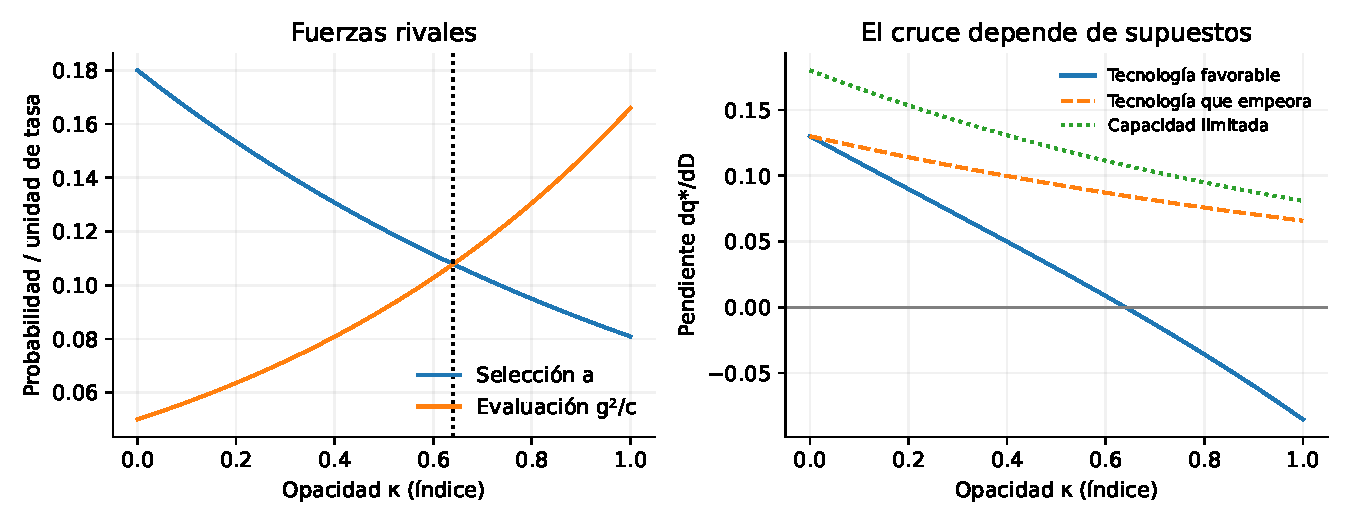
\includegraphics[width=\linewidth,height=.65\textheight,keepaspectratio]{../code/figures/mechanisms.pdf}
\par\small Caso favorable: $\kappa^*=\threshold$. Caso de tecnología que empeora y caso de capacidad limitada: sin pendiente negativa.
\source{Simulaciones hipotéticas de code/verify.py. Sin estimación con datos peruanos.}
\end{frame}

% Exposición estimada: 60 segundos.
\begin{frame}{Esquinas: el candidato interior puede fallar}

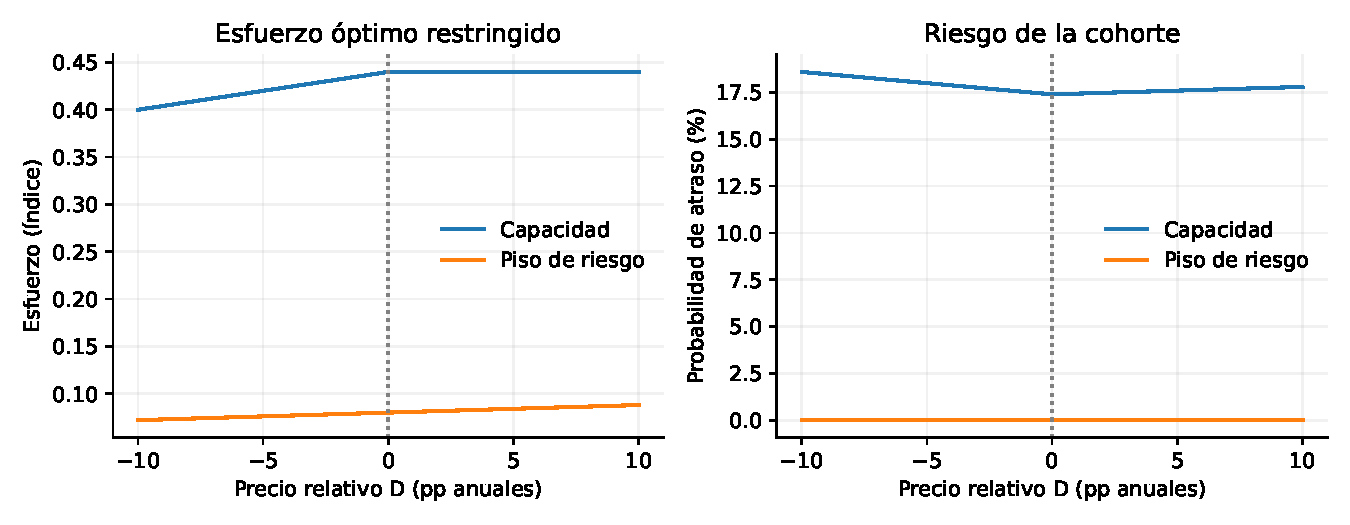
\includegraphics[width=\linewidth,height=.66\textheight,keepaspectratio]{../code/figures/corners.pdf}
\par\small En la restricción de capacidad, la pendiente pasa de $-0.12$ a $0.04$. El piso de riesgo detiene reducciones adicionales.
\source{Parámetros ilustrativos. code/verify.py contrasta solución analítica y optimización acotada independiente.}
\end{frame}

% Exposición estimada: 75 segundos.
\begin{frame}{De una cohorte al saldo total}

Fijemos el mismo evento de atraso y horizonte $h$.
$M(D)$: fracción total de cartera en atraso. Una cohorte agrupa créditos nuevos.
\begin{itemize}
\item $B_0>0$: saldo antiguo. $m_0\in[0,1]$: su fracción en atraso.
\item $B(D)>0$, diferenciable: saldo de la cohorte nueva todavía vigente.
\item $w(D)=B(D)/(B_0+B(D))$: peso nuevo.
\end{itemize}
\[
M(D)=\frac{B_0m_0+B(D)q^*(D)}{B_0+B(D)}=(1-w)m_0+wq^*.
\]
\small S5: saldos deterministas o población continua, maduración compatible, sin castigos ni selección adicional por amortización. $B_0,m_0$ fijos al variar precio.
\end{frame}

% Exposición estimada: 80 segundos.
\begin{frame}{Proposición 3: calidad y composición}

Bajo S1--S3 y S5, donde $q^*$ es diferenciable, sea $\beta_D=\partial_Dq^*$.
Desde aquí, la prima indica derivada respecto del precio $D$.
\[
\boxed{M'=\underbrace{w\beta_D}_{\text{calidad de lo nuevo}}
+\underbrace{w'(q^*-m_0)}_{\text{composición}}.}
\]
\begin{itemize}
\item Si $w'=0$, el signo se conserva.
\item Si $\beta_D\ne0$ y $|w'(q^*-m_0)|<w|\beta_D|$, también se conserva.
\end{itemize}
Si $B=B_1\exp(-\varepsilon D)$: $B_1>0$ es el saldo en $D=0$ y $\varepsilon\ge0$ su sensibilidad proporcional. Entonces $w'=-\varepsilon w(1-w)$.
\[
M'=w[\beta_D-\varepsilon(1-w)(q^*-m_0)].
\]
\end{frame}

% Exposición estimada: 80 segundos.
\begin{frame}{Contraejemplo: signos opuestos válidos}

En $D=0$, $q^*=0.225$, $m_0=0.10$, $\beta_D=0.13$, $w=0.20$ y $\varepsilon=3$.
\[
M'=0.2[0.13-3(0.8)(0.225-0.10)]=\stockSlope<0.
\]
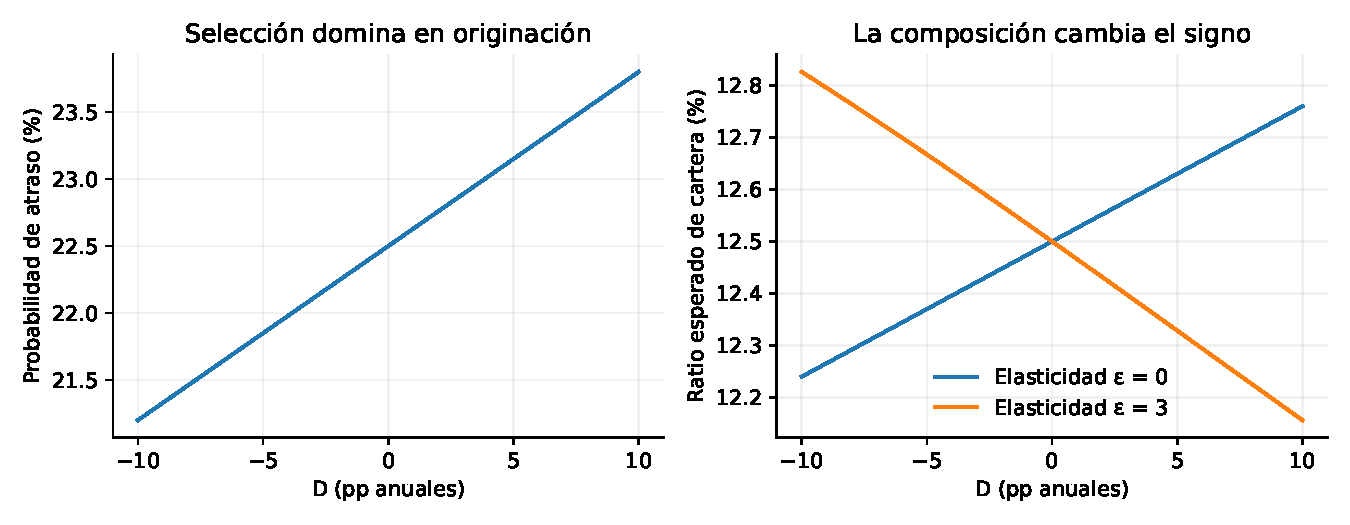
\includegraphics[width=\linewidth,height=.43\textheight,keepaspectratio]{../code/figures/stock_composition.pdf}
\source{Ejemplo hipotético. El riesgo nuevo empeora, pero disminuye su peso en una cartera antigua más segura.}
\end{frame}

% Exposición estimada: 65 segundos.
\begin{frame}{Sensibilidad y alcance de las comprobaciones}

\begin{columns}[T,onlytextwidth]
\column{.55\textwidth}
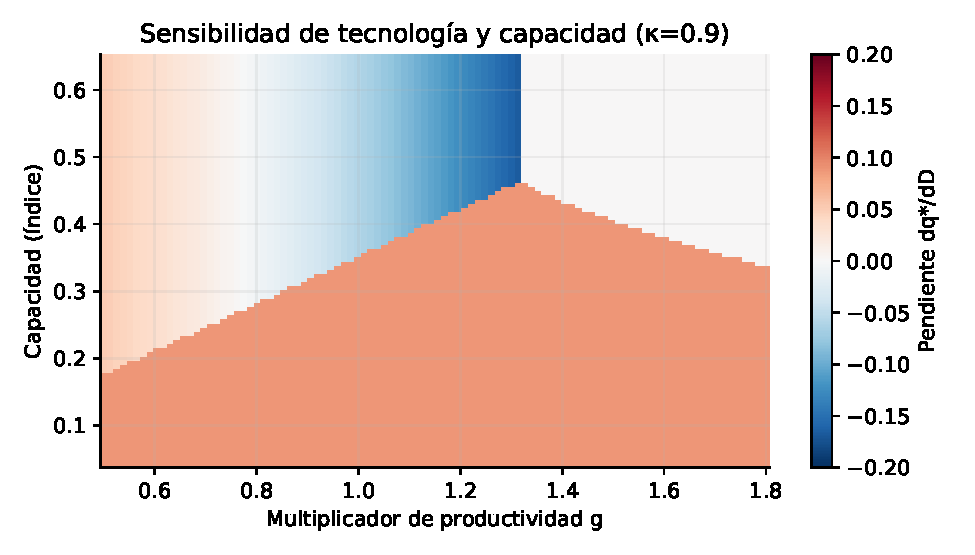
\includegraphics[width=\linewidth,height=.62\textheight,keepaspectratio]{../code/figures/sensitivity.pdf}
\column{.42\textwidth}
\small
\begin{itemize}
\item 1495 sorteos válidos: interior, capacidad y piso.
\item Optimizador independiente, diferencias finitas y SymPy.
\item Dominios y contraejemplos provocan fallas si no se cumplen.
\end{itemize}
\par\medskip
Una malla encuentra errores. No prueba un teorema ni utilidad predictiva empírica.
\end{columns}
\source{code/verify.py, semilla 20261110. Parámetros ilustrativos.}
\end{frame}

% Exposición estimada: 95 segundos.
\begin{frame}[fragile]{Lean: pruebas generales y cierre en curso}
\small
\textbf{Artículo, identidad de P3:} $M=(1-w)m_0+wq^*$.
\par\smallskip
\textbf{Enunciado y prueba reales} de esa cláusula en Lean:
\begin{lstlisting}[basicstyle=\ttfamily\footnotesize,escapeinside={(*@}{@*)}]
theorem portfolioRatio_eq_weighted (B0 m0 : (*@$\mathbb R$@*))
    (B q : (*@$\mathbb R \to \mathbb R$@*)) (D : (*@$\mathbb R$@*)) (hden : B0 + B D (*@$\ne$@*) 0) :
    portfolioRatio B0 m0 B q D =
      (1 - cohortWeight B0 B D) * m0 +
        cohortWeight B0 B D * q D := by
  unfold portfolioRatio impairedBalance cohortWeight
  field_simp
  ring
\end{lstlisting}
\texttt{portfolioRatio} es $M$; \texttt{cohortWeight} es $w$.
El denominador no nulo se deriva de los saldos positivos de S5.
\par\smallskip
\textbf{Estado:} P1--P3 compilan sin admisiones. Falta el cierre oficial.
Sin hipótesis matemáticas añadidas; no verifica datos ni causalidad.
\source{Prueba en Galarza26RelativeCredit/Stock.lean; fuente, hashes y estado vigente: docs/lean\_progreso.md.}
\end{frame}

% Exposición estimada: 80 segundos.
\begin{frame}{Una afirmación de IA revisada críticamente}

\small
Respuesta heredada de octubre, traducida: ``El modelo está cerrado como un problema bancario de dos etapas.''
\par\medskip
\textbf{Veredicto: incompleta.} La FOC interior no resuelve restricciones ni la etapa de precios.
\[
\pi_e=0\Rightarrow z=gR/c,\qquad
e^*=\min\{z,\bar e,q^0/g\}.
\]
La derivación por cuadrado completo permite revisar el paso sin confiar en la IA.
\par\medskip
\textbf{Manuscrito real pendiente.} No se recibieron páginas escritas por el autor.
La guía en \texttt{hand/} desglosa cada manipulación para escribirla y digitalizarla.
\source{Registro histórico preservado en prompts.md. Guía tipográfica no presentada como manuscrito.}
\end{frame}

% Exposición estimada: 50 segundos.
\begin{frame}{Próximo contraste predictivo}

\begin{itemize}
\item Base: morosidad pasada y ciclo. Ampliación: precio relativo.
\item Entrenar solo con resultados ya publicados en cada origen.
\item Pesos y escalas con pasado, mismas fechas para ambos modelos.
\item Comparar pérdidas fuera de muestra y estabilidad por periodo.
\end{itemize}
\par\medskip
No se recibió el panel reproducible del plan. No reporto RMSE, valores $p$ ni mejoras estimadas.
\source{Plan de Grados y Galarza. Clark y West (2007), para modelos anidados bajo sus condiciones.}
\end{frame}

% Exposición estimada: 65 segundos.
\begin{frame}{Qué está demostrado y qué queda abierto}

\begin{itemize}
\item \textbf{Demostrado en el texto:} solución global, umbral condicionado y transmisión con composición.
\item \textbf{Paso difícil:} conectar una probabilidad de cohorte con un ratio de saldo y resolver esquinas.
\item \textbf{Abierto:} precios de equilibrio y utilidad predictiva peruana. El cierre oficial de Lean sigue en curso.
\item \textbf{Trabajo personal:} derivaciones manuscritas, comprensión y ensayo oral.
\end{itemize}
\par\medskip
Costos, garantías, castigos y exposición cambiaria pueden alterar la señal.
\end{frame}

% Exposición estimada: 45 segundos.
\begin{frame}{Conclusión para supervisión}

\Large
Una tasa relativa se interpreta junto con la evaluación y la renovación de la cartera.
\normalsize\bigskip
\begin{itemize}
\item La condición $a-g^2/c$ rige dentro del régimen interior.
\item El saldo agrega calidad y composición.
\item La utilidad del indicador requiere prueba fuera de muestra.
\end{itemize}
\end{frame}

% Exposición estimada: 45 segundos.
\begin{frame}{Preguntas para la clase}

\begin{enumerate}
\item ¿Qué medida observable permitiría distinguir mayor evaluación de cambios en la calidad de solicitantes?
\item ¿Conviene comenzar con cosechas o con ratios de saldo, dadas las fuentes públicas peruanas?
\item ¿Qué contraste separaría una respuesta de evaluación de una caída en el peso de créditos nuevos?
\end{enumerate}
\bigskip
\href{https://github.com/fgalarzac/ai-project/tree/apoyo}{Código, artículo y estado de los componentes}

\end{frame}
\end{document}
